
\section{Architektur}
\label{sec:Architektur}
% Vorgehen nach C4 Modell

\subsection{Systemkontext}
\label{architektur:Systemkontext}
% KOntext Diagramm

\subsection{Container}
\label{architektur:Container}

\subsubsection{QGIS Plugin}
\label{architektur:QGIS Plugin}


\subsubsection{Plaza Vorverarbeitung}
\label{architektur:Plaza Vorverarbeitung}

Für unser optimiertes Routing wird in regelmässigen Abständen der neueste \ac{OSM}-Datensatz\cite{osm_data_switzerland} der Schweiz geladen. Bevor die Daten einer Routing-Engine zur Verarbeitung in einen Routing-Graph übergeben werden, sollen zuerst unsere optimierten Pfade als Wege in die Flächen eingepflegt werden. Abbildung \ref{fig:workflow_vorverarbeitung} zeigt diesen Ablauf schematisch auf. Im Folgenden werden die einzelnen Komponenten der Vorverarbeitung besprochen.

\begin{figure}[ht]
\centering
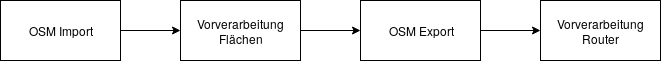
\includegraphics[width=1\linewidth]{projectdoc/img/workflow_vorverarbeitung.png}
\caption[Ablauf Vorverarbeitung]{Ablauf der Vorverarbeitung der \ac{OSM}-Daten bis zur Übergabe an den Router; Grafik erstellt mit \emph{draw.io}}
\label{fig:workflow_vorverarbeitung}
\end{figure}

\paragraph{OSM Import}~\\
Die \acs{OSM}-Import Komponente liest das komplette für uns relevante Kartenmaterial (z.B. die Schweiz) als \ac{PBF} ein und sucht dabei nach Flächen, die wir bearbeiten wollen.

Dazu werden \emph{Osmium} und die dazugehörigen Python-Bindings \emph{pyOsmium}\cite{pyosmium} verwendet. Osmium erkennt automatisch Flächen aus \ac{OSM} Multipolygone oder Relationen. Mit einem eigenen Handler können wir dabei gleich das Einlesen des Files auf die für uns interessanten Flächen beschränken, wie in Listing \ref{osmium_import_code} gezeigt wird.

\begin{listing}[ht]
    \inputminted{python}{projectdoc/listing/osmium_handler.py}
    \caption[Einlesen OSM-Daten mit Osmium]{Einlesen von OSM Daten mithilfe von \emph{Osmium}; Filterung auf für uns relevante Flächen}
    \label{osmium_import_code}
\end{listing}

\paragraph{Vorverarbeitung der Flächen}\label{par:Vorverarbeitung der Flächen}~\\
Die mit Osmium importierten \ac{OSM}-Daten sind noch reine \ac{OSM}-Objekte, auf denen keine Geometrie-Berechnungen angewendet werden können. Dazu wird die Python-Library \emph{Shapely}\cite{shapely} verwendet. Shapely kann mit Geometrien umgehen und Algorithmen von \ac{GEOS} wie \code{intersection} und \code{contains} darauf anwenden.

Um die mit Osmium importierten Objekte in Shapely zu verwenden, werden diese ins \ac{WKB} Format übersetzt und Shapely übergeben, wie in Listing \ref{shapely_import_code} gezeigt.

\begin{listing}[ht]
    \inputminted{python}{projectdoc/listing/shapely_import.py}
    \caption[Einlesen OSM Objekte in Shapely]{Übergabe von Osmium-Objekten zu Shapely für die Weiterverarbeitung}
    \label{shapely_import_code}
\end{listing}

\paragraph{OSM Export}~\\
Die durch unseren Algorithmus erzeugten Wege durch Flächen (in Shapely Datenstrukturen) sollen nun wieder zurück ins \ac{OSM}-Format geschrieben werden. Die bisher erwähnten Libraries bieten eine solche Funktion leider nicht an. Auch sonst ist zum Zeitpunkt dieser Arbeit keine stabile Library dafür auffindbar. Die Erklärung dafür liegt wohl darin, dass beim Extrahieren der Geometrie (siehe Absatz \nameref{par:Vorverarbeitung der Flächen}) alle Meta-Daten (z.B. Tags) von \ac{OSM} verloren gehen. Bei der umgekehrten Konvertierung (Geometrie zu \ac{OSM}) müssen also wieder Meta-Daten hinzugefügt werden. Diese Problematik kann ein generisches Konvertierungs-Tool nicht ohne weiteres lösen.

Für diese Komponente wird daher eine eigene Implementation geschrieben, die jediglich Wege aus Geometrien in ein \ac{OSM}-Format schreibt und mit den für uns relevanten Meta-Daten versieht.

\subsubsection{Plaza Routing}
\label{architektur:Plaza Routing}

\paragraph{nächste ÖV-Haltestellen finden}~\\
\label{architektur:nächste ÖV-Haltestellen finden}

Das grundlegende Ziel ist es von einem Startpunkt aus eine Destination zu Fuss und mit dem öffentlichen Verkehr zu erreichen. Dabei sollen die ÖV-Haltestellen in einem zu Fuss machbaren Umkreis berücksichtigt werden. Von diesen Haltestellen ausgehend wird das ÖV-Routing an die Zieldestination durchgeführt.

Für die Anforderung \ref{target:nächste ÖV-Haltestellen finden} bietet sich Overpass an. Overpass ermöglicht es über eine umfassende \ac{API} selektiv Daten von \ac{OSM} zu beziehen. Dabei besteht die Option, die Overpass \ac{QL} oder XML-Abfragen zu verwenden. Die Suche lässt sich nach allem einschränken, was der Mapper in den \ac{OSM}-Daten spezifizieren kann. So ist das Filtern nach Objekttyp, Keys, Tags, etc. unbeschränkt möglich und bietet so eine hohe Flexibilität. Overpass liefert die Resultate als JSON-Objekt oder XML. 

Für eine einfache Intergration in Python gibt es Overpass Wrapper. Dabei wurden zwei Libraries berücksichtigt, namentlich overpass-api-python-wrapper und OverPy. Die Libraries haben einen ähnlich häufigen Updatezyklus. Für beide wurde ein Proof of Concept implementiert, welcher die ÖV-Haltestellen im einem kleinen Umkreis vom Stadelhofen, Zürich, Schweiz abfragt.

Die Entscheidung fiel dabei auf OverPy. Ausschlaggebend war die ausführlichere Dokumentation und dass OverPy Klassen für Nodes, Relations, Way, Area, etc. und Hilfsfunktionen, welche das Ganze übersichtlich halten, anbietet. Bei overpass-api-python-wrapper besteht der Nachteil, dass das JSON-Resultat der Abfrage selber geparsed und verarbeitet werden muss.

\begin{listing}[ht]
    \inputminted{python}{projectdoc/listing/get_public_transport_stops_overpass.py}
    \caption{ÖV-Haltestellen von \acs{OSM} mit Overpass beziehen}
    \label{get_public_transport_stops_overpass}
\end{listing}

In Listing \ref{get_public_transport_stops_overpass} ist zu sehen, wie für eine Bounding Box, welche im Süden durch den minimalen Breitengrad, im Westen durch den minimalen Längengrad, im Norden durch den maximalen Breitengrad und im Osten durch den maximalen Längengrad begrenzt ist, die ÖV-Haltestellen abgefragt werden. Dabei wird die JSON-Response in Node-Objekte geparsed, welche weiterverwendet werden können. In diesem Beispiel wird für die Abfrage die erwähnte Overpass QL verwendet.

Es ist ebenfalls möglich, eine Umkreissuche mit \code{around}  durchzuführen. Dies hat Performance-Nachteile und es gibt keine entscheidenden Gründe, warum es vorteilhafter sein sollte, wenn man einen Kreis statt ein Rechteck um einen Ausgangspunkt zieht.

\subsubsection{Router}
\label{architektur:Router}

TODO
